\section{Background and Applications}
\label{sec:background}

\begin{figure*}
\begin{func}[$\Func_{\textsc{com}}$]
    $\Func_{\textsc{com}}$ proceeds as follows, running with parties $A$ and
  $B$, and an adversary $S$.
    \begin{enumerate}
        \item Upon receiving a message $(\mathsf{Commit}, b)$ from $A$, where $b
          \in \{ 0, 1 \}$, record the value $b$ and send the message
          $(\mathsf{Receipt})$ to $B$ and $S$. Ignore any subsequent
          \textsf{Commit} messages.
        \item Upon receiving a message $(\mathsf{Open})$ from $A$, proceed as
          follows: If some value $b$ was previously recorded, then send the
          message $(\mathsf{Open}, b)$ to $B$ and $S$ and halt. Otherwise, halt.
    \end{enumerate}
\end{func}
\caption{An ideal functionality for a one-time commitment scheme.}
\label{func:com}
\end{figure*}

Security in the UC framework is based on the real world/ideal world paradigm,
also known as simulation-based security. In the real world, a set of parties
executes the protocol in a distributed fashion as defined by its model. In the
ideal world, the parties securely access an \emph{ideal functionality} $\mc{F}$,
which is imagined as an incorruptible third party that securely (by definition)
carries out the task to be achieved by the protocol. The idea is that $\mc{F}$
obtains inputs from the parties, runs the program that carries out the task, and
returns outputs back to the parties.

For example, Figure~\ref{func:com} describes an ideal functionality
$\Func_{\textsc{com}}$ for a one-time commitment scheme, which allows a party
$A$ to commit to some hidden value $b$ and later reveal it to a party $B$. In
particular, a commitment scheme should satisfy two properties: 1) the committed
value $b$ should be hidden from $B$ prior to revealing (the \emph{hiding}
property), and 2) $A$ should only be able to commit and reveal a single value
(the \emph{binding} property). It should be clear that $\Func_{\textsc{com}}$
captures these properties in the ideal world, but in the real world, where the
ideal functionality does not exist, the goal is to construct a commitment scheme
that is ``just as good as'' $\Func_{\textsc{com}}$.

We say that the protocol \emph{securely realizes} (or \emph{emulates}) $\mc{F}$
if any attack that is possible on the protocol is also possible on $\mc{F}$. But
since we have designed $\mc{F}$ to be secure by definition, such an attack does
not lead to a break in security. Proving emulation formally proceeds in two
steps. The first step is constructive: We must construct a \emph{simulator}
$\mc{S}$ (a simulated adversary) that can emulate the attack of any adversary
$\mc{A}$ on the protocol, but instead, on $\mc{F}$. The second step is a
relational analysis: We must show that running the protocol under attack by any
adversary $\mc{A}$ (the real world) is \emph{indistinguishable} from running
$\mc{F}$ under attack by $\mc{S}$ (the ideal world) to any distinguisher
$\mc{Z}$, called the \emph{environment}. In particular, $\mc{Z}$ is an
interactive distinguisher: it interacts with the real world and the ideal world
in a well-defined manner, and the simulation is good if no $\mc{Z}$ can
distinguish between the two. Figure~\ref{fig:uc-experiment} illustrates the UC
experiment: connecting lines denote communication channels,\footnote{Note that
  all communication passes through the adversary $\mc{A}$. In the bare model,
  communication is asynchronous, unauthenticated, and unreliable, but other
  models of communication can be built atop this model.} $P_1, P_2, \ldots, P_n$
represent parties executing the real protocol, and $D_1, D_2, \ldots, D_n$ represent
``dummy'' parties that simply relay information between the environment and the
ideal functionality.

The advantage of security definitions in UC is that they satisfy strong
composability guarantees, even under concurrent composition. Suppose that $\pi_1$
is a protocol that securely realizes a functionality $\mc{F}_1$. If a protocol
$\pi_2$, using $\mc{F}_1$ as a subroutine, securely realizes a functionality
$\mc{F}_2$, then the protocol $[\pi_1 / \mc{F}_1]\pi_2$, in which calls to
$\mc{F}_1$ are replaced by calls to $\pi_1$, also securely realizes
$\mc{F}_2$. That way, it suffices to analyze the security of the standalone
protocol $\pi_2$ in the $\mc{F}_1$-hybrid model, where parties run $\pi_2$ with
access to $\mc{F}_1$, as opposed to the composite protocol of $\pi_2$ and
$\pi_1$. Figure~\ref{fig:uc-composition} illustrates protocol composition: the
setup on the left represents the $\mc{F}_1$-hybrid model, and the setup on the
right represents the protocol substitution $[\pi_1 / \mc{F}_1]\pi_2$, which
maintains security.

\begin{figure}
  \centering
  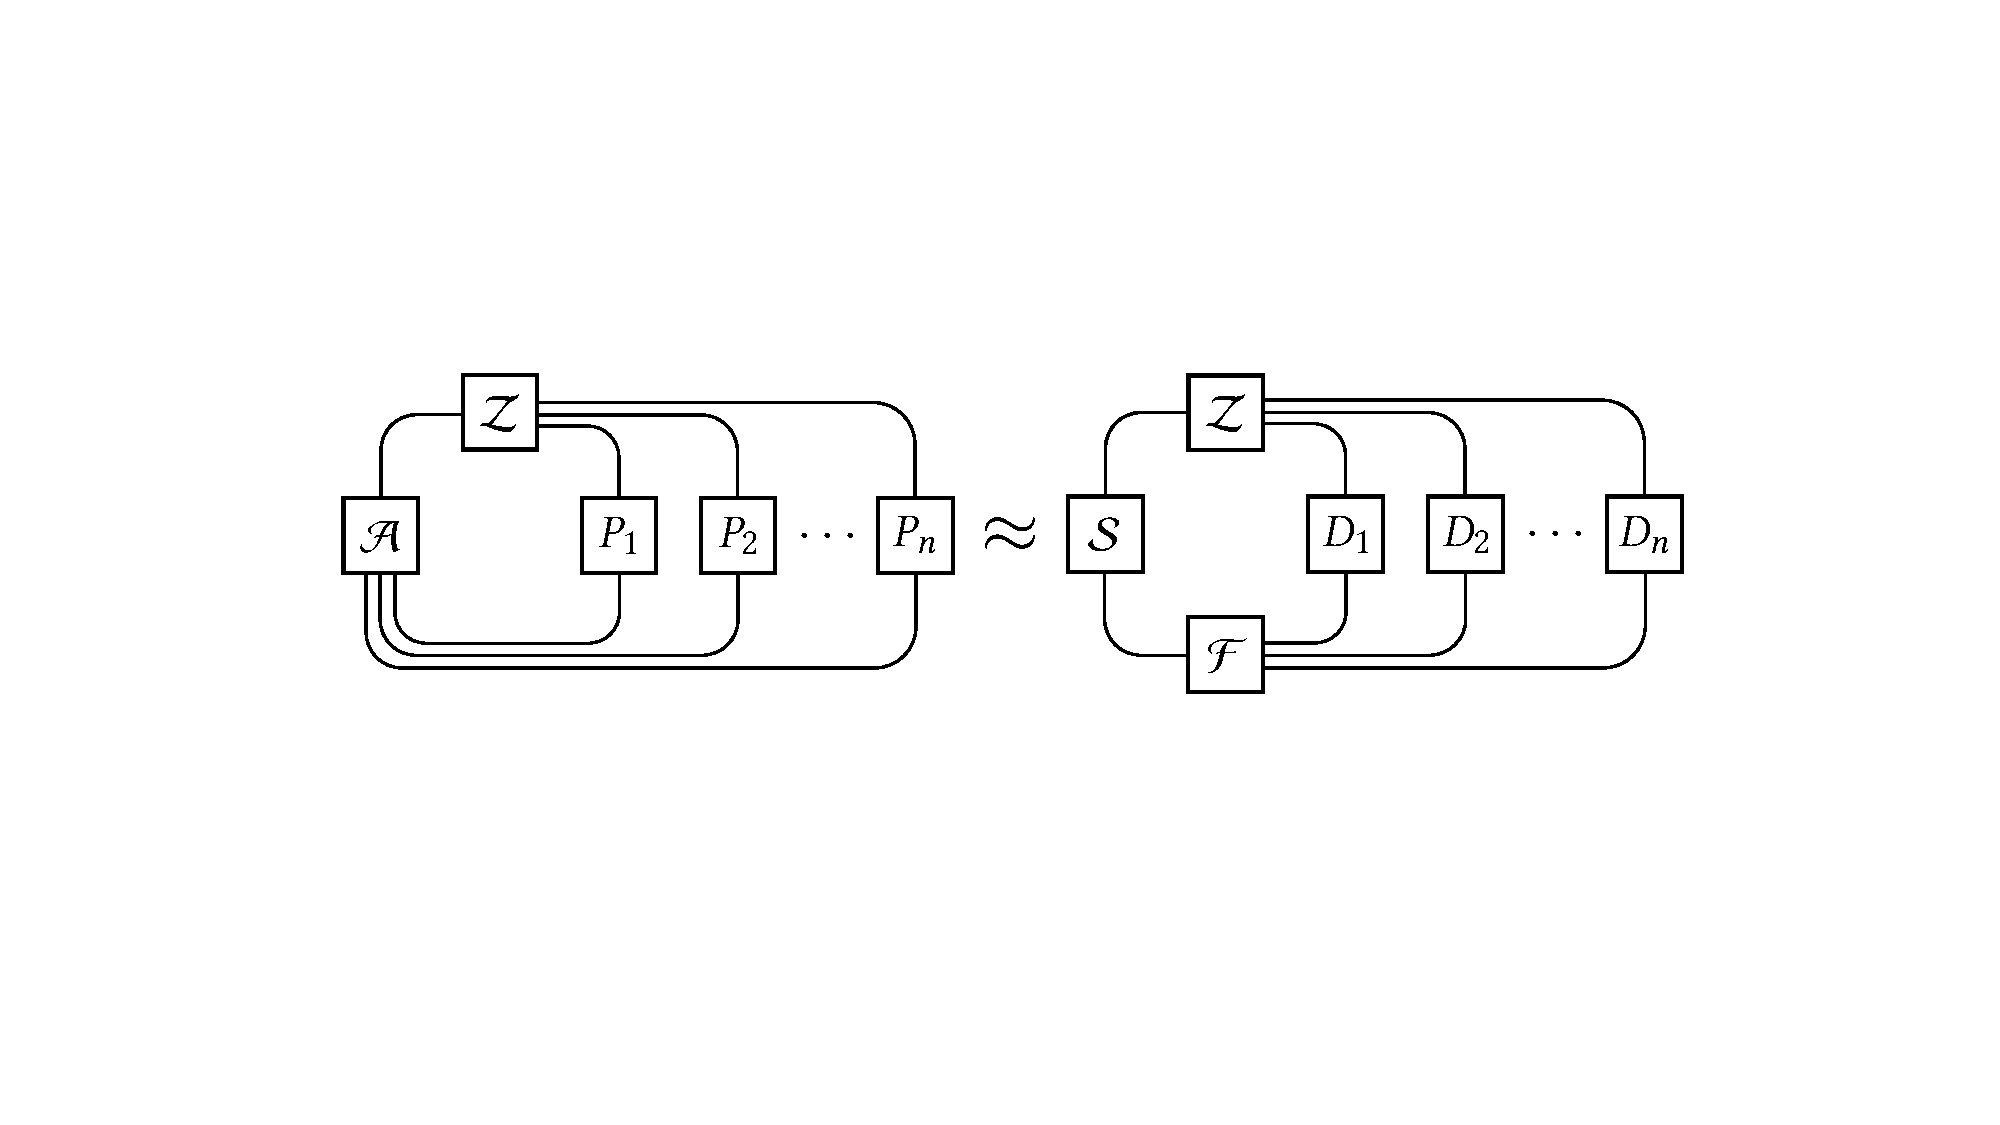
\includegraphics[width=\linewidth]{graphics/uc-experiment}
  \caption{UC experiment with real world (left) and ideal world (right).}
  \label{fig:uc-experiment}
\end{figure}

\begin{figure}
  \centering
  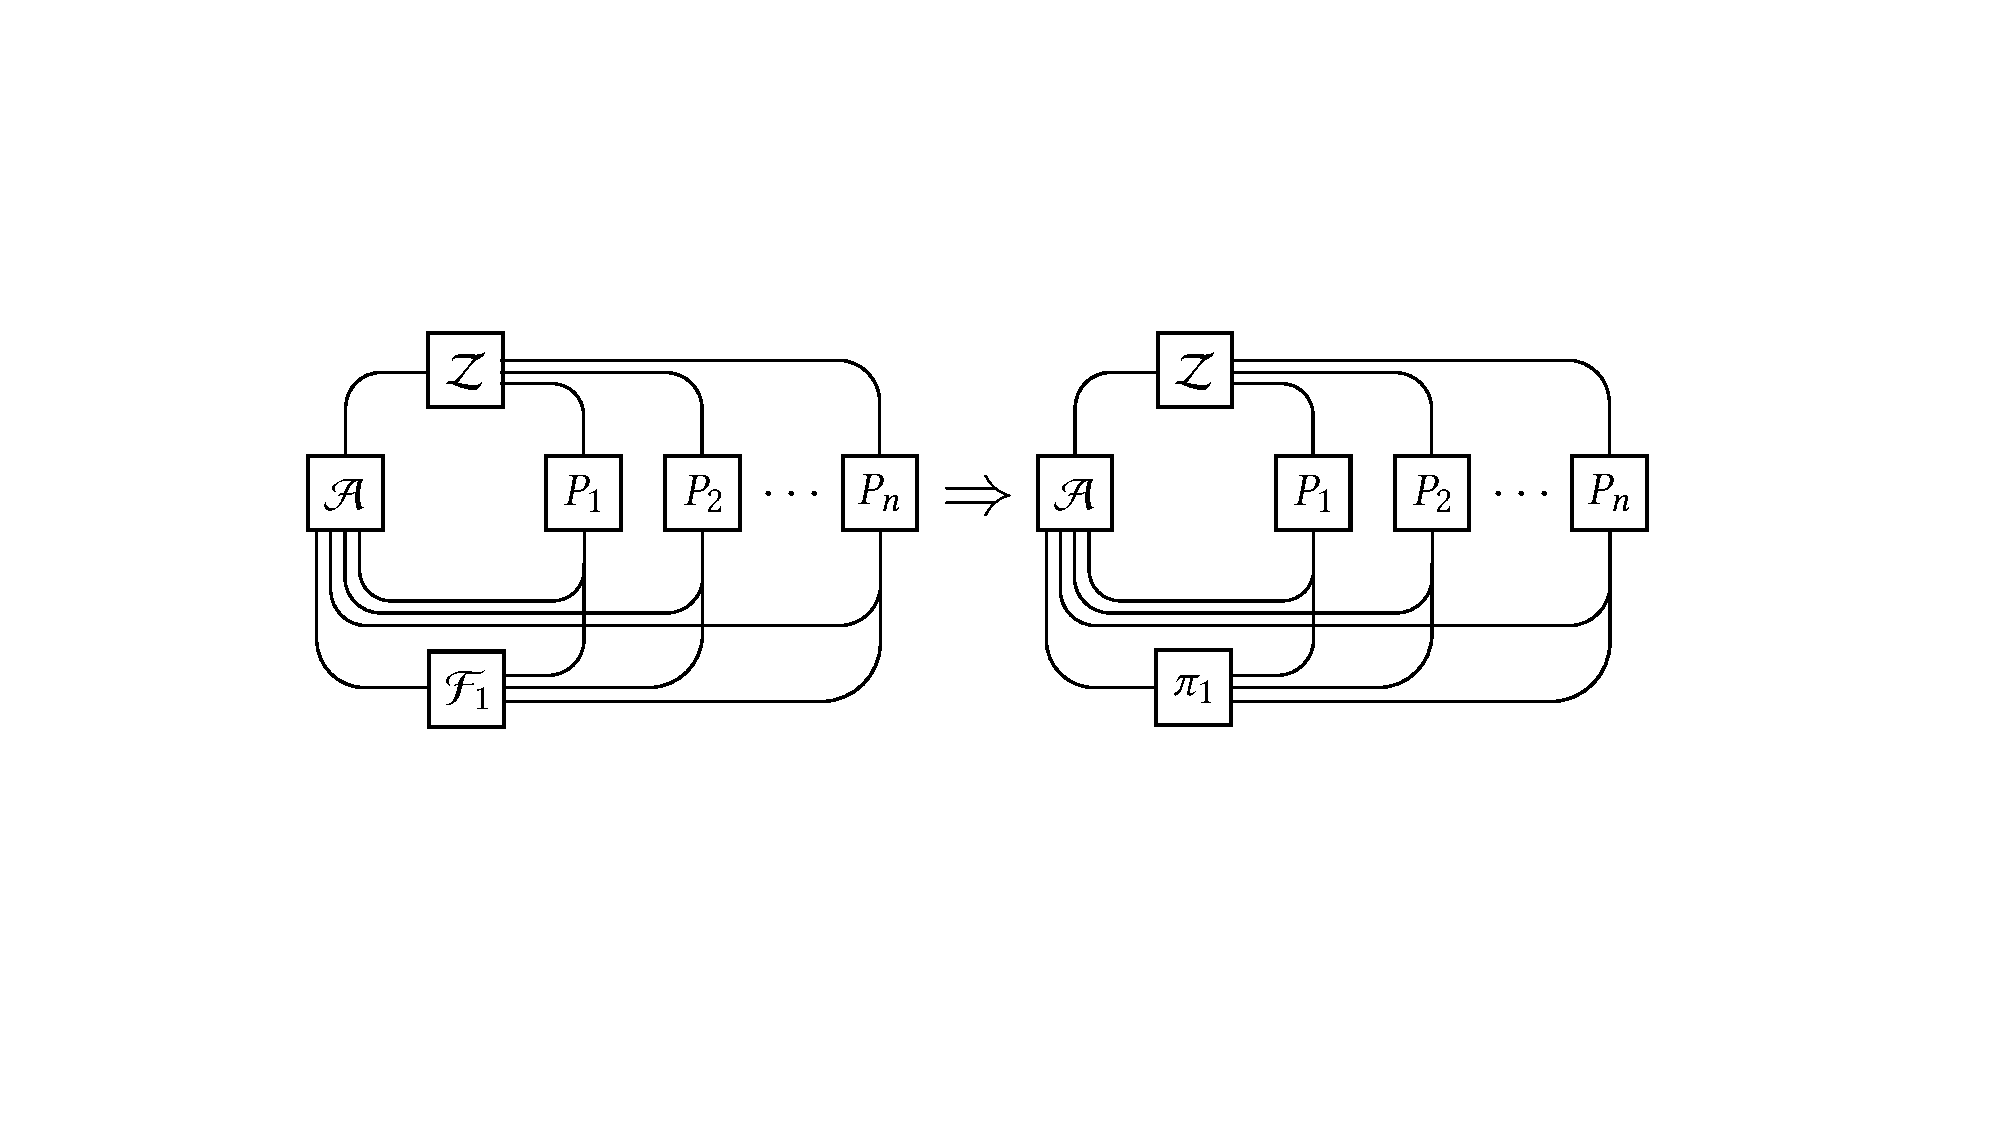
\includegraphics[width=\linewidth]{graphics/composition}
  \caption{UC protocol composition theorem.}
  \label{fig:uc-composition}
\end{figure}
